
\chapterbegin{Metodología a usar}

\section{Desarrollo y Metodología Ágil}

El desarrollo de software es un proceso cuyo objetivo es la creación de un programa informático para la resolución de un problema o para obtener una funcionalidad deseada. Este proceso es muy extenso y suele incluir varias etapas, incluyendo, pero no limitandose a: 

\begin{itemize}
	\item{\textbf{Estudio del problema}. Dónde se estudia y analiza la tarea en cuestión, detallando la solución deseada.}
	
	\item{\textbf{Detalle de las especificaciones}. Es necesario descomponer el problema para describir todas las posibles restricciones y condiciones de funcionamiento.}
	
	\item{\textbf{Diseño}. En esta etapa se crea una representación de qué forma va a tener el programa informático a desarrollar teniendo en cuenta las especificaciones.}
	
	\item{\textbf{Programación}. En este momento es cuando se creará el código especifico del programa siguiendo el diseño anterior.}
	
	\item{\textbf{Documentación}. Es el proceso de crear la información que acompaña al programa para describir su funcionamiento y ayudar a su mantenimiento, tanto a nivel de usuario como a nivel de desarrollador.}
	
	\item{\textbf{Testeo}. Fase de pruebas en la que se comprueba que el programa funciona como es debido, no tiene errores y cumple con las especificaciones.}
	
	\item{\textbf{Mantenimiento}. Fase final del desarrollo en la que se da soporte a la aplicación, manteniéndola actualizada y arreglando fallos no detectados anteriormente.}
	
	
\end{itemize}


Estas etapas están claramente diferenciadas y en el desarrollo clásico se siguen de forma secuencial, pero en la actualidad se siguen las llamada metodologías ágiles, que permiten un desarrollo mucho más rápido, detectando errores antes y obteniendo un producto para el cliente en menos tiempo. Es común utilizar un modelo iterativo (véase figura \ref{fig:MU_modeloiterativo}), en el que estas fases se repiten tras obtener una retroalimentación del cliente, en lugar de dar fin al desarrollo. 


\begin{figure}
	\centering
	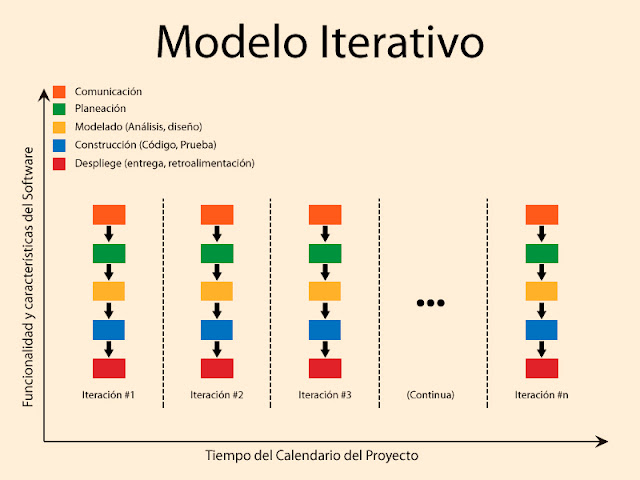
\includegraphics[width=0.5\textwidth]{03.EstudioProblema/04.MetodologiaAUsar/00.Figuras/01.modelo_iterativo.jpg}
	\caption{Diagrama de desarrollo iterativo. \cite{MU_img_modeloiterativo}}
	\label{fig:MU_modeloiterativo}
\end{figure}


El proceso evolutivo es similar y en ocasiones complementario al iterativo, ya que al final de cada iteración, se obtiene parte del resultado final, sobre el que en iteraciones posteriores se irán añadiendo funcionalidades. (véase figura \ref{fig:MU_modeloevolutivo})


\begin{figure}
	\centering
	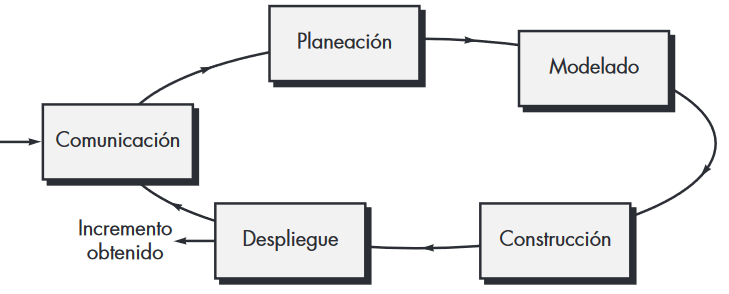
\includegraphics[width=0.5\textwidth]{03.EstudioProblema/04.MetodologiaAUsar/00.Figuras/02.modelo_evolutivo.png}
	\caption{Diagrama de desarrollo evolutivo. \cite{MU_img_modeloevolutivo}}
	\label{fig:MU_modeloevolutivo}
\end{figure}

 
Tanto el modelo iterativo como el evolutivo permiten un desarrollo centrado en el usuario, ya que el cliente final proporciona información sobre los desarrollos ya entregados que permiten mejorar constantemente. Además de dar seguridad al equipo desarrollador de que su próximo trabajo tiene una base sólida, evitando tener que rehacer trabajo en una fase muy avanzada al descubrir un problema.

Por estos motivos, para este proyecto se va a utilizar una metodología evolutiva basada en entregas, obteniendo al final de cada entrega una parte funcional del producto final. La organización de estas entregas, así como las especificaciones para cada una de ellas se describen en detalle en la sección \textbf{Plan de Entregas} (\ref{sec:planentregas}) y todo su contenido en la parte \textbf{Desarrollo} (\ref{sec:desarrollo}).

Para el caso particular de desarrollo de videojuegos se siguen las mismas metodologías que para cualquier otro software, pero adquiere especial importancia un documento llamado Game Design Document, donde se detalla toda la información del videojuego final.

\section{Game Design Document}

El Game Design Document o GDD es un documento en constante evolución que describe de la forma más detallada posible todos los aspectos de un videojuego. Al ser un documento especifico para este tipo de desarrollos, permite alcanzar gran profundidad sobre todo de información del juego.  Por norma general este documento se crea en colaboración entre todos los equipos de personas que trabajan en la creación del proyecto, desde programadores hasta artistas conceptuales o diseñadores de jugabilidad. El documento suele crearse antes de comenzar el desarrollo pero está abierto a actualizarse y añadir nueva información durante el proceso de desarrollo.

La función principal de este documento es plasmar la visión que tienen los equipos del producto final y servir de guía a todos ellos para alcanzar el objetivo de la forma deseada. También puede tener la función de carta de presentación entre un equipo de desarrollo y una editorial cuando los primeros buscan financiación.

Para el desarrollo de este proyecto se ha creado un GDD simplificado y adaptado a las particularidades de este Trabajo de Fin de Grado. El documento se encuentra en el apéndice \textbf{Game Design Document} (\ref{sec:apendice:GDD}).

\section{Evaluación}
\label{sec:evaluacion}

Una parte importante para este proyecto es evaluar el juego creado y su usabilidad obteniendo datos a partir de pruebas con usuarios reales. La usabilidad es un aspecto fundamental en el desarrollo de software y habitualmente es definida como una métrica usada para evaluar la facilidad de uso del producto, su efectividad, eficiencia y la satisfacción que produce en los usuarios. \cite{MU_eval_usabilidad}

Existen varios métodos para medir la usabilidad de un sistema, los heurísticos y los empíricos. Los primeros se basan en conocimientos teóricos para analizar detalladamente el funcionamiento de una aplicación. Por otra parte, los métodos experimentales se centran en obtener información de usuarios del programa. La forma más común es a través de cuestionarios de satisfacción o SUS (System Usability Scale).

Los cuestionarios SUS son usados en diversos ámbitos a parte del desarrollo software y son un estándar que permite evaluar la eficacia, eficiencia y satisfacción que proporciona cualquier sistema. Estos cuestionarios cuentan con diez enunciados cuidadosamente diseñados a los que se responde con un número del 1 al 5 (1 - Totalmente en desacuerdo y 5 - Totalmente de acuerdo). De esta forma se puede aplicar una sencilla fórmula matemática para obtener un resultado numérico indicando el grado de usabilidad del sistema. \cite{MU_eval_sus}

Los diez enunciados se dividen en 5 positivos y 5 negativos, intercalados entre sí. Para obtener la puntuación final hay que seguir estos pasos:


\begin{itemize}
	\item{Sumar los resultados de los enunciados positivos y restar 5.}
	
	\item{Restar a 25 la suma de los enunciados negativos.}
	
	\item{Por último, sumar los dos números anteriores y multiplicar el resultado por 2,5.}

\end{itemize}

Como resultado se obtiene un número entre 0 y 100. Cuanto mayor sea el número, mejor será la usabilidad del sistema. Por norma general se entiende que un resultado aceptable debe ser superior a 68 puntos. (figura \ref{fig:MU_sus})


\begin{figure}
	\centering
	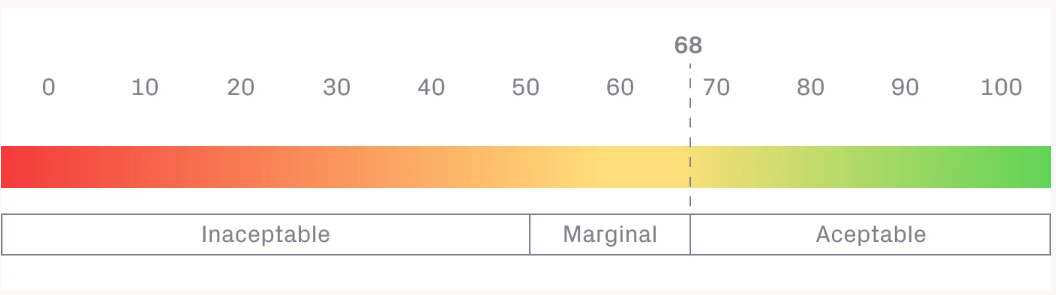
\includegraphics[width=0.5\textwidth]{03.EstudioProblema/04.MetodologiaAUsar/00.Figuras/03.sus.png}
	\caption{Representación de los resultados de un SUS. \cite{MU_eval_sus}}
	\label{fig:MU_sus}
\end{figure}


Se ha elegido el cuestionario SUS como método para realizar la evaluación de este proyecto principalmente por tratarse de una herramienta estándar en el sector, por su simplicidad para los usuarios que tienen que rellenarlo y por dar un resultado numérico fácilmente interpretable. El cuestionario utilizado junto con sus resultados se encuentra en el apéndice \textbf{Cuestionarios} (\ref{sec:apendice:Custionarios}) 


















\chapterend